\documentclass[xcolor=pdftex,dvipsnames,table,10pt,babel]{beamer}

\usetheme{Warsaw}

\usepackage[spanish]{babel}
\usepackage[latin1]{inputenc}
\usepackage{stmaryrd}
\usepackage{graphicx}

\usepackage{listings}


\usepackage{setspace}

\usepackage{color}
\usepackage{textcomp}
\definecolor{listinggray}{gray}{0.9}
\definecolor{lbcolor}{rgb}{0.95,0.95,0.95}
\lstset{
    backgroundcolor=\color{lbcolor},
    tabsize=4,
    rulecolor=,
    language=matlab,
        basicstyle=\scriptsize,
        upquote=true,
        aboveskip={1.5\baselineskip},
        columns=fixed,
        showstringspaces=false,
        extendedchars=true,
        breaklines=true,
        prebreak = \raisebox{0ex}[0ex][0ex]{\ensuremath{\hookleftarrow}},
        frame=single,
        showtabs=false,
        showspaces=false,
        showstringspaces=false,
        identifierstyle=\ttfamily,
        keywordstyle=\color[rgb]{0.1,0.1,0.6}\bfseries,
        commentstyle=\color[rgb]{0.133,0.545,0.133},
        stringstyle=\color[rgb]{0.627,0.126,0.941},
}


\setbeamercovered{transparent}

\title{FuD: A Framework for Small Distributed Projects}
\author{Guillermo Biset}
\pgfdeclareimage[height=2.5cm]{unrc}{images/escudo.jpg}
\pgfdeclareimage[height=2.5cm]{fudepan}{images/logo-fudepan.png}

\institute[U.N.R.C.]{
  \textsc{Departamento de Computaci\'on} \\
  \textsc{Universidad Nacional de R\'io Cuarto} \\
  \ \\
  \pgfuseimage{unrc}  \qquad \qquad \qquad \pgfuseimage{fudepan}}

\date{}

\begin{document}

\frame{\titlepage}

\frame{
\frametitle{Temario: }
\tableofcontents
}

\section{Motivation}

\subsection{FuD}

        \frame{
            \frametitle{Motivation}
            \begin{block}{}
            The use of computational resources traverses most of the applied sciences.
            \end{block}

            \pause
            
            \begin{block}{}
            Many of these uses present high processing requirements and handle large data sets.
            \end{block}

            \pause
            
            \begin{block}{}
            A good approach is to use parallelization techniques in computing to handle these sets.
            \end{block}
            
            \pause
            
            \begin{block}{}
            The \textbf{problem}, however, is that most of the scientist with the correct amount of domain-specific knowledge are not necessarily prepared for parallel programming.
            \end{block}

        }

        \frame{
          \frametitle{Motivation 2}
          
          It is necessary to develop an application framework that allows non-advanced programmers to implement applications where:
          \begin{itemize}
          \item The use of the framework exploits the benefits of parallel computing.
          \pause
          \item No previous knowledge of parallel programming (or concurrency) is required.
          \pause
          \pause
          \item The use of te framework doesn't impose serious performance drawbacks.
          \pause
          \item The framework must exploit different (and dynamic) layouts of the computational resources.
          \end{itemize}
        }

    \begin{frame}
     \frametitle{Similar Approaches}
     
     Several approaches deal with some of these properties:
     
     \begin{block}{}
     \begin{description}
     \item [BOINC]: Is a non commercial middleware designed at Berkeley for volunteer and grid computing\cite{boinc1}.
     \pause
     \item [MPI]: Is an API that allows many computers to communicate among themselves, primarily used in High Performance Clusters\cite{mpi}.
     \pause
     \item [MapReduce]: Is a programming model developed at Google to improve the implementation of distributed algorithms\cite{mapreduce}.
     \end{description}

     \end{block}

    \end{frame}

\subsection*{C++}

\begin{frame}[fragile]
  \frametitle{C++}

C++ is a statically typed, multi paradigm, compiled and general purpose language. It is considered a middle-level language, since it provides both low-level primites and high-level constructs.

The following is a code snippet from FuD.

\lstset{language=C++}
\begin{lstlisting}[frame=single]
//exception if _ids_to_job_map[id] isn't defined
mili::find(_ids_to_job_map,id)->process_results(id, message);

//remove from pending list
std::list<JobUnit*>::iterator it;
it = find_if(_pendingList.begin(),_pendingList.end(), 
             boost::bind(&JobUnit::get_id, _1) == id);

if (it != _pendingList.end())
{
    delete *it;
    _pendingList.erase(it);
}
else
    syslog(LOG_NOTICE,"Finished JobUnit % u was not pending.",id);
\end{lstlisting}


\end{frame}

\section{FuD}

    \frame{
      \frametitle{\textbf{F}uDePAN \textbf{U}biquitous \textbf{D}istribution}
      
      The following goal summarizes the target of the FuD framework:
      
      \pause
      
      \begin{block}{}
      Design and develop a framwork to automate the distribution of computer applications throughout heterogenous and dynamic processing nodes.
      \end{block}
      
      \pause
      
      Also, this design should:
      \begin{itemize}
       \item Be flexible as to allow the development of any application.
       \pause
       \item Be independent of the resources that would be available during the projects lifetime.
       \pause
       \item Be flexible to avoid constraining itself to a particular communication model between nodes.
      \end{itemize}

    }

    \frame{
      \frametitle{Summarizing}
      
      FuD can be used to solve any problem that can be solved sequentially. Also, the implementer:
      
      \begin{itemize}
      \item Doesn't need to know parallel programming.
      \pause
      \item Is not restricted to a particular layout of processing nodes.
      \pause
      \item Is not restricted to a particular communication model.
      \end{itemize}

      \pause

      Finally, \textbf{FuD} ensures:
      \begin{itemize}
      \item The application has the potential to execute in parallel.
      \pause
      \item The application will exploit availabe resources at any given time.
      \pause
      \item The use of the framework won't mean significant performance loss (comparing with other implementations).
      \pause
      \item Exchanged data between server and client applications won't carry a significant burden on top of the necessary data.
      \end{itemize}

    }

  \subsection{Concepts}

  \frame{
    \frametitle{\textbf{FuD} Concepts}
    
    \textbf{FuD} is organized in a Master-Worker (one server, several connected clients) scheme. The following concepts help understand the framework's behaviour:
    
    \begin{description}
    \item[Client]: An application connected to the server handling processing tasks.
    \pause
    \item[DistributableJob]: An abstract task to be performed by an application. It can be further subdivided into \emph{JobUnit}s.
    \pause
    \item[JobUnit]: A concrete unit of work to be performed, it can't be divided.
    \pause
    \item[ClientsManager]: The module in charge of handling connected clients.
    \pause
    \item[JobManager]: The module in charge of handling both types of jobs.
    \end{description}

  }

  \subsection{Approach}

  \frame{
    \frametitle{Approach}
    
    To ensure this, it is necessary to implement a \emph{Divide\&Conquer} scheme, where processing is taken care of by the processing nodes (clients):
    
    \pause 
    
    \begin{block}{\emph{Divide\&Conquer + Process}}
    \begin{description}
     \item [Divide]: A \emph{DistributableJob} is divided into \emph{JobUnit}s. This is a transactional process. Implemented in \texttt{produce\_next\_job\_unit(size)}.
     \pause
     \item [Conquer]: Once the results of a \emph{JobUnit} are computed, they are handled by \texttt{handle\_results(id, input)}.
     \pause
     \item [Process]: Work units are passed to connected clients. They will be in charge of processing them and then returning the results for handling.
    \end{description}

    \end{block}

  }

  \subsection{Overview}

  \frame{
    \frametitle{Layers of the framework}
    
    \textbf{FuD} is divided into 3 well separated layers:
    
    \begin{center}
    \includegraphics [height=5cm]{images/abslayers.jpg}
    \end{center}
  }
  
  \frame{
    \frametitle{Layers of the framework}
    
    \begin{description}
    \item[Application]: Provides components regarding aspects of the problem's domain. As such, includes data definition and handling code relevant to the problem.
    \pause
    \item[Job Management]: In charge of dealing with jobs during their life span, bonding concrete application distributable jobs to the clients that will handle their job units for processing.
    \pause
    \item[Communication]: The only real link between master and worker applications, will handle connection and communication issues.
    \end{description}

  }

  \frame{
    \frametitle{Clusterer: Class Diagram}

    \begin{center}
      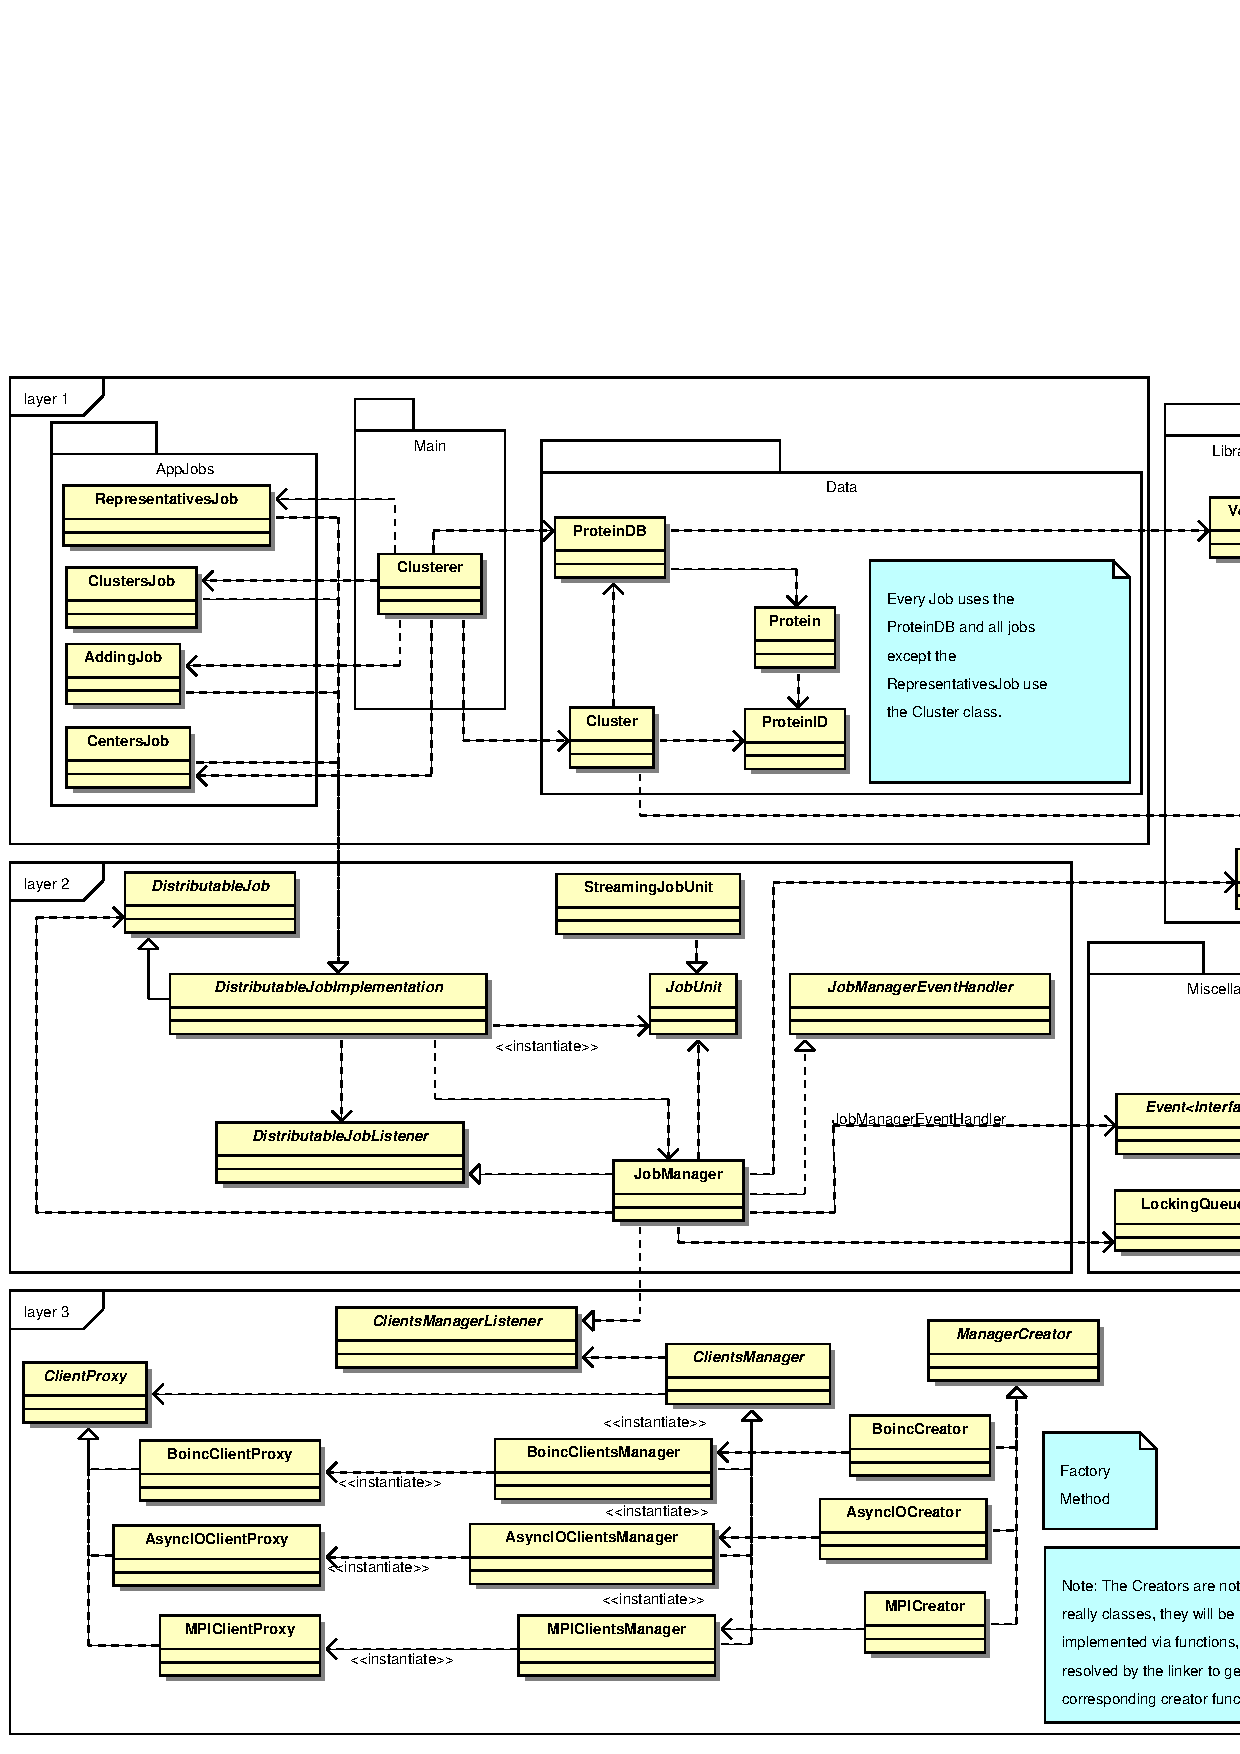
\includegraphics[height=7cm]{images/server-cd.jpg}
    \end{center}

  }

  \frame{
    \frametitle{Clusterer: Client Class Diagram}
    
    \begin{center}
    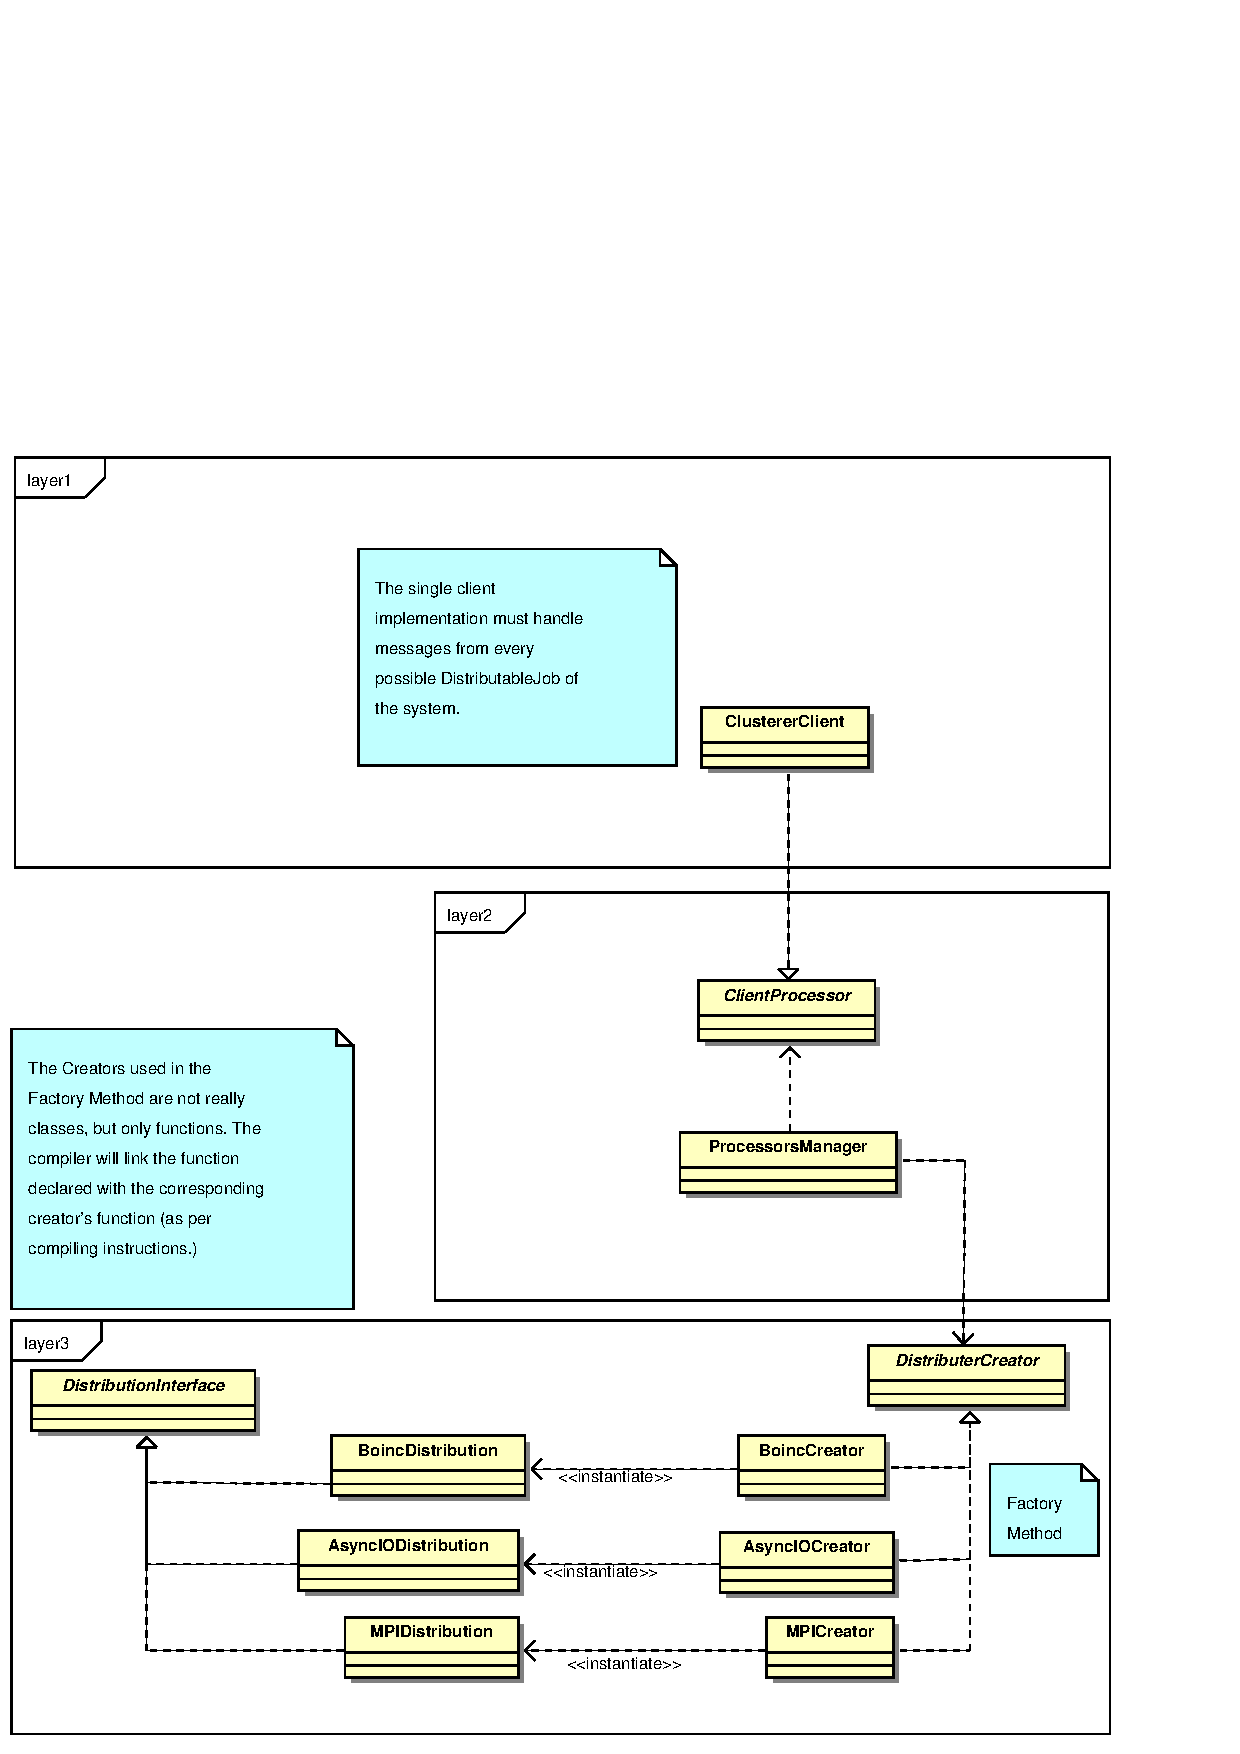
\includegraphics[height=7cm]{images/client-cd.jpg}
    \end{center}
  }

\subsection{Implementation}

\frame{
  \frametitle{How does a \textbf{FuD} application work?}
  
  The main app. uses \textbf{FuD} the following way:
  
  \begin{enumerate}
   \item Creates concrete \texttt{DistributableJob} instances.
   \pause
   \item Uses the methods in the \texttt{DistributableJob} interface:
     \begin{description}
     \item[run()]: Executes or start the job.
     \pause
     \item[wait\_completion()]: Waits for job completion (blocking).
     \end{description}
  \end{enumerate}
  \pause
  Also, the app. implementer must:
  \begin{itemize}
   \item Define the jobs' name (for logging purposes).
   \pause
   \item Define the jobs' state (such as \emph{FinishedGenerating}).
   \pause
   \item Define a method for subdivision.
   \pause
   \item Define a method for result handling.
  \end{itemize}

}

\begin{frame}[fragile]
\lstset{language=C++}
\begin{lstlisting}[frame=single]
#include "counter.h"
#include "getopt_pp.h"

using namespace fud; using namespace GetOpt;

int main(int argc, char** argv) {
  size_t number(1000);
  size_t jobs_n(5);

  GetOpt_pp ops(argc, argv);
  ops >>Option('n',"number", number) >>Option('j',"jobs",jobs_n);

  NumberDatabase* db = new NumberDatabase(number);

  std::vector<Counter*> jobs;
  for (size_t i(0); i < jobs_n; ++i)
    jobs.push_back( new Counter(*db,i) );

  for (size_t i(0); i < jobs_n; ++i)
    jobs[i]->run();

  jobs[jobs_n-1]->wait_completion();

  std::cout << "Last num: " << db->current_number() << std::endl;
}
\end{lstlisting}

\end{frame}

\frame{
  \frametitle{How does a \textbf{FuD} application work?}
  
  \begin{center}
  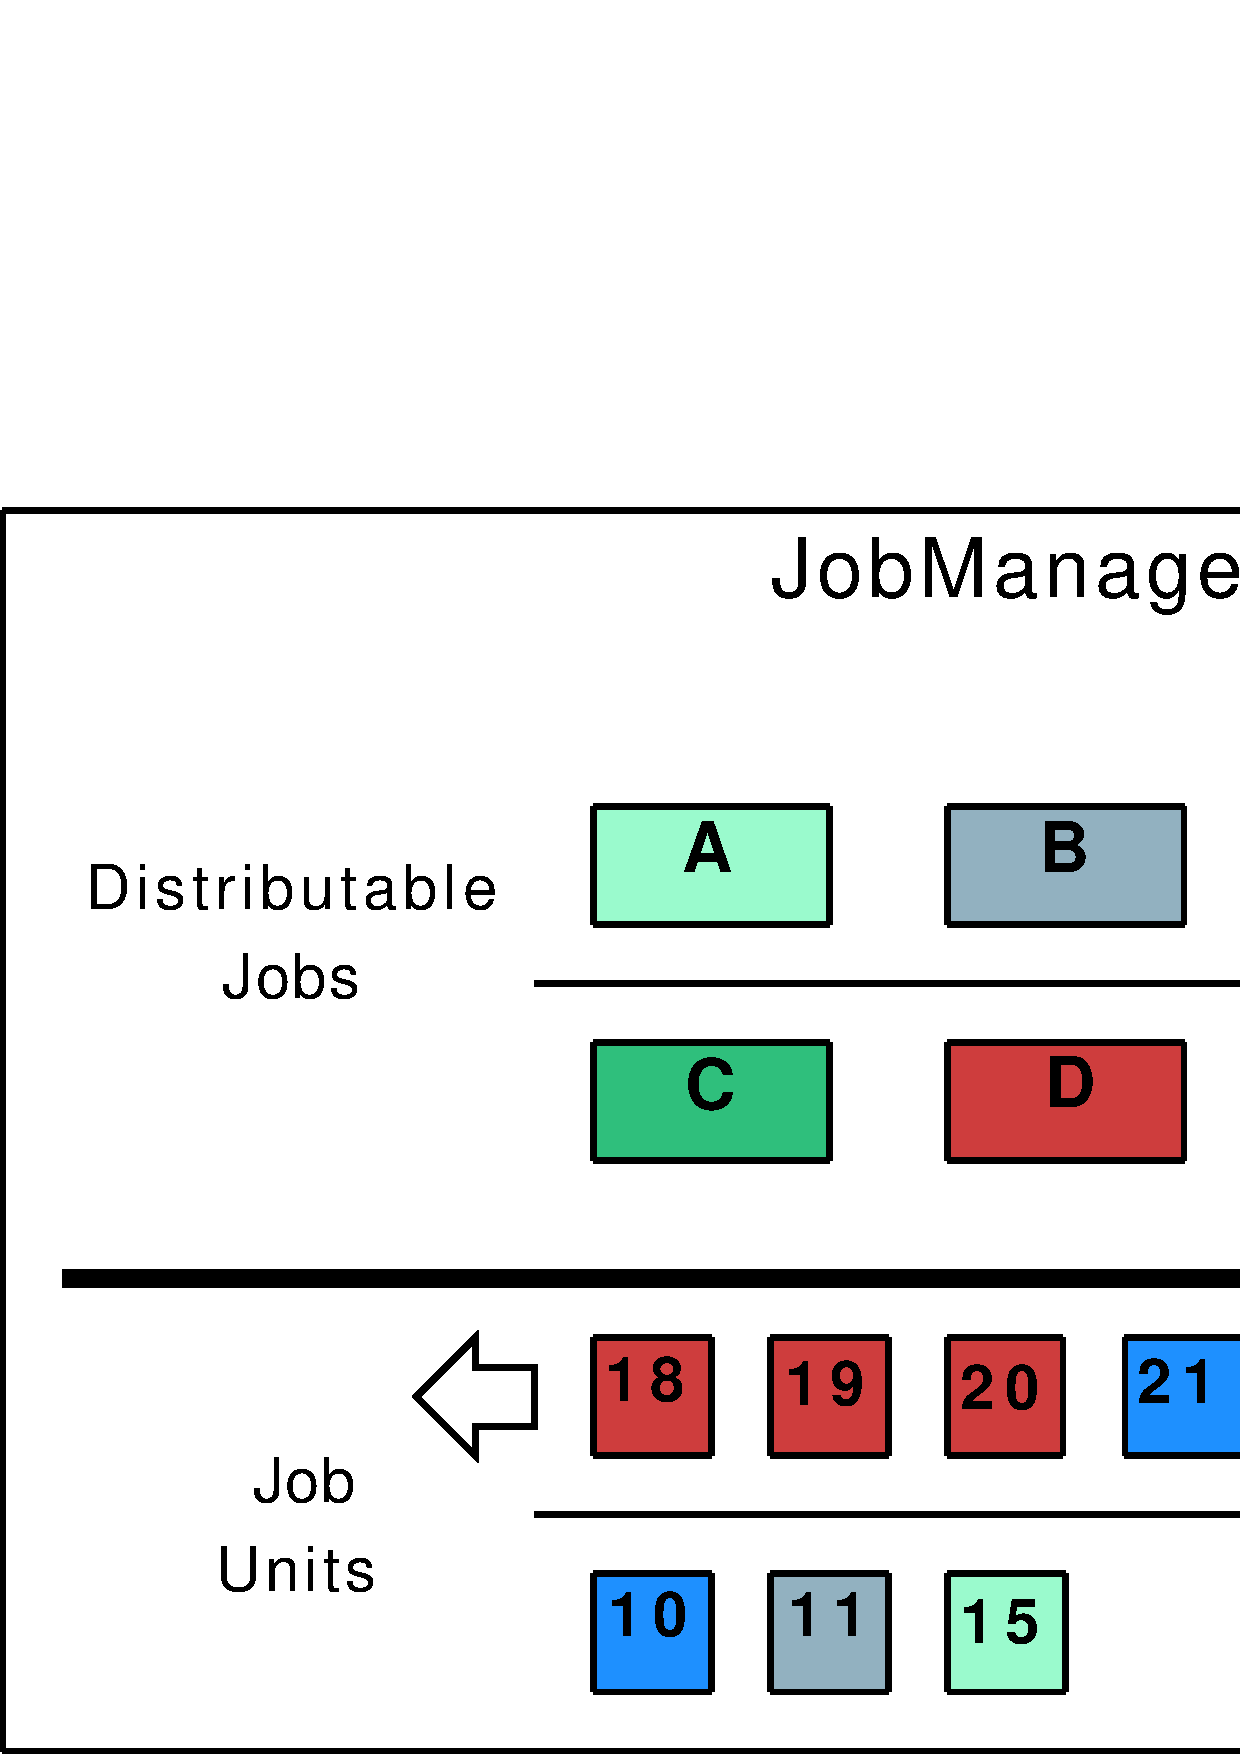
\includegraphics[height=5cm]{images/JobManager.jpg}
  \end{center}

} 

\section{Extending FuD}

\subsection{New Communication Layer}

\frame{
  \frametitle{Extending the communication layer}
  
  As of now, the FuD framework uses an asynchronous input-output library from boost.
  
  However, it is a good idea to extend the framework to use other communication models.
  
  To do this, one must implement a descendant of \texttt{ClientsManager} and \texttt{ClientProxy} (server side) and a concrete \texttt{DistributionClient} (client side). These are shown in red in the following diagram:

  \begin{center}
    \includegraphics [height=4.5cm]{images/redl1.jpg}
  \end{center}

}

\subsection{Steps}

\frame{
  \frametitle{Step 1: A concrete Clients Manager}
  
  Remember: it is the \texttt{ClientsManager}'s instance responsibility to connect clients and create the corresponding proxies.
  
  It is not necessary for the implementer to code the handling itself, just the connection and sending procedures:
  
  \pause
  
  \begin{block}{Implementing the \texttt{ClientsManager} descendant}
    \begin{enumerate}
     \item Include headers \texttt{clients\_manager.h} and \texttt{client\_proxy.h}.
     \pause
     \item In the constructor you should start a server to listen for incoming connections.
     \pause
     \item When a new client is connected, simply create your own \texttt{ClientProxy} (see next slide) instance and call \texttt{register\_client}.
     \pause
     \item Optionally reimplement \texttt{get\_available\_client()} if you wish to execute some internal heuristic procedure to decide the client you will use.
    \end{enumerate}

  \end{block}

}

\frame{
  \frametitle{Step 2: A concrete Client Proxy}
  
  The proxy acts as a representative (in the server side) of a connected client.
  
  The implementation must be able to answer for the state of the client and handle communication with it.
  
  \pause
  
  \begin{block}{Implementing the \texttt{ClientProxy} }
    \begin{enumerate}
      \item For design purposes, the descendant proxy should be implemented as private class of your clients manager.
      \pause
      \item Only two methods must be implemented:
      \begin{description}
        \item[busy]: Returns true if the client is not ready to handle more work.
        \pause
        \item[process]: Send a \texttt{JobUnit} to the client.
      \end{description}
    \end{enumerate}
 
  \end{block}

  \pause
  
  And that's all, the rest of the work is on the client side.
}

\frame{
  \frametitle{Step 3: The client side}

  Things are easier on the client side, the implementer must only implement a concrete \texttt{DistributionClient}:
  
  \pause
  
  \begin{block}{Implementing a \texttt{DistributionClient} }
  \begin{enumerate}
    \item Include header \texttt{distribution\_client.h}.
    \pause
    \item Implement the following methods:
    \begin{description}
    \item[void inform\_result(bool result)]: Informs the results back to the proxy.
    \pause
    \item[virtual void run()]: Should attempt to connect to the server.
    \end{description}
  \end{enumerate}
  \end{block}

}

\section{The Road Ahead}

\begin{frame}
\frametitle{Future Work}

\begin{block}{}
\begin{itemize}
 \item Compilation using autotools.
 \pause
 \item Development of a BOINC implementation.
 \pause
 \item Development of an MPI implementation.
 \pause
 \item Support for multi-threaded clients.
 \pause
 \item Availability to handle several job units per client at a time.
 \pause
 \item Development of abstract application layers and subsequent instances.
\end{itemize}
\end{block}
\end{frame}


\begin{frame}[allowframebreaks]{Bibliography} 
\bibliography{biblio}
\bibliographystyle{apalike}
\end{frame} 

	\frame {
		\centerline{\Huge{\textbf{?`Preguntas?}}}
	}

\frame {
    \centerline{\Huge{\textbf{Gracias}}}
}

    \frame{
      \cite{parallel}
      \cite{svn}
      \cite{tnssitl}
      \cite{texknuth}
      \cite{latex}
      \cite{oosc}
      \cite{design}
      \cite{pressman}
      \cite{async}
      \cite{faulttolerance}
      \cite{mapreduce}
      \cite{flynn}
      \cite{cplusplus}
      \cite{boinc1}
      \cite{boinc2}
      \cite{sched1}
      \cite{tanenbaum1}
      \cite{tanenbaum2}
      \cite{sched2}
      \cite{loadbal}
      \cite{uml}
      \cite{softwarepractices}
      \cite{mpi}
      \cite{openmp}
      \cite{ewd1036}
      \cite{responsibility}
      \cite{boost}
    }

\end{document}

